% --- SIDE-BY-SIDE FIGURES (SHARING PAGE WIDTH) ---
\begin{figure*}[!t]
  \centering
  % Left Side: Dataset Samples
  \begin{minipage}{0.48\textwidth}
    \centering
    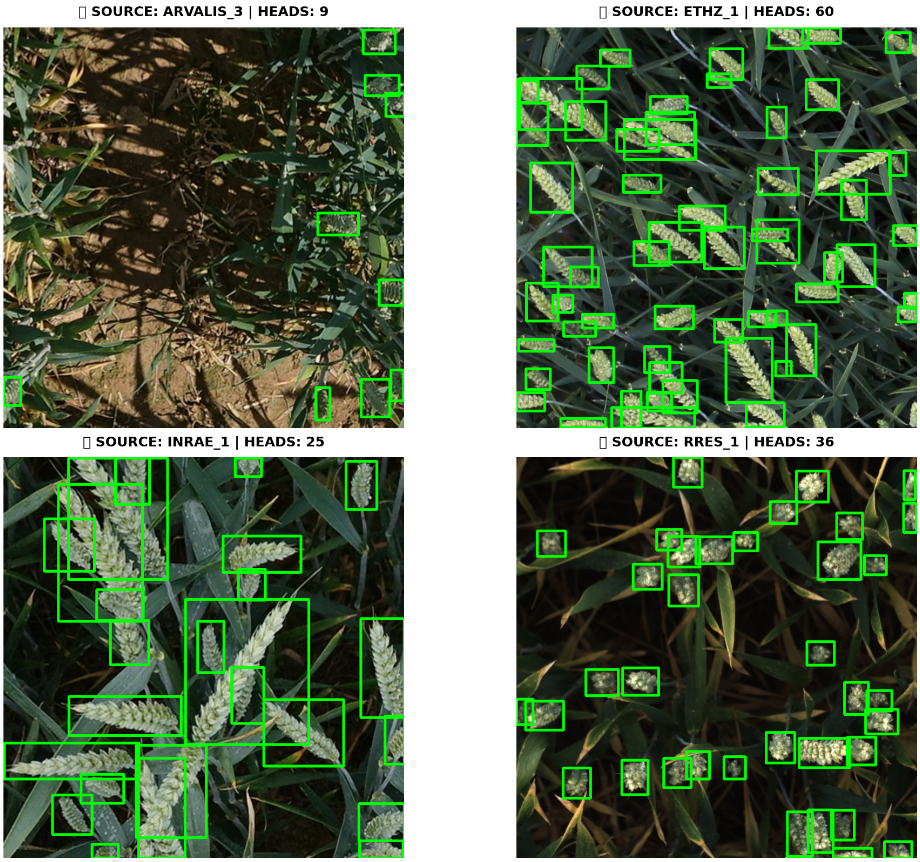
\includegraphics[width=\linewidth]{wheat_variance.png}
    \caption{Diverse environmental conditions present in the training dataset, showcasing extreme variations in plant density, background soil color, and ambient lighting.}
    \label{fig:dataset_variance}
  \end{minipage}
  \hfill % Adds space between the two images
  % Right Side: Architecture Diagram
  \begin{minipage}{0.48\textwidth}
    \centering
    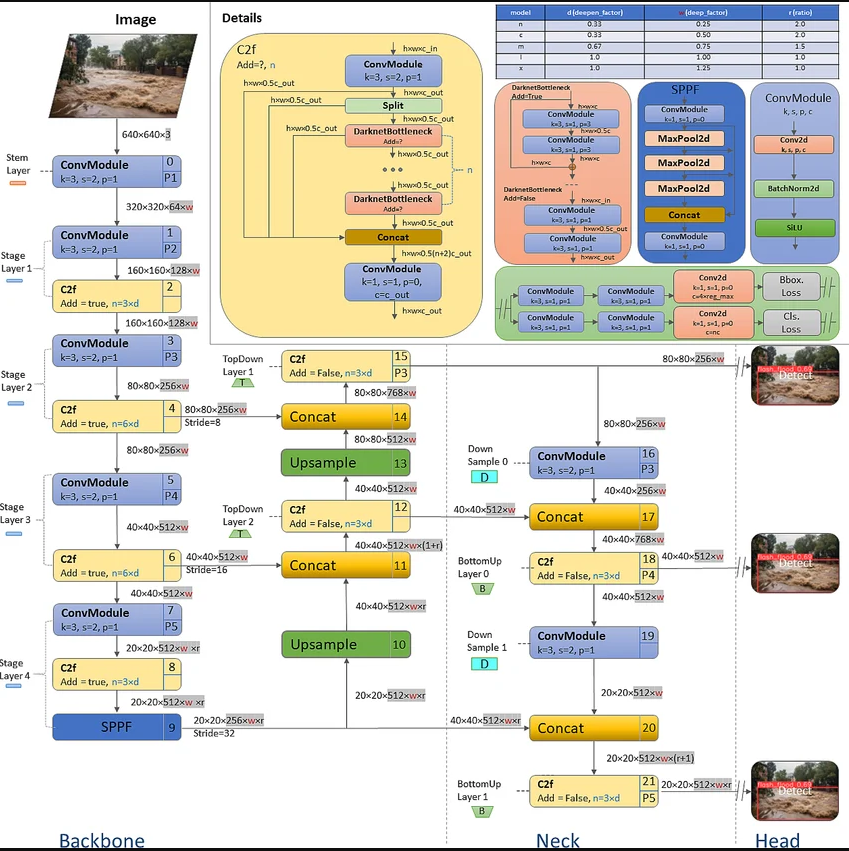
\includegraphics[width=\linewidth]{sec/yolov8s_1.png}
    \caption{Structural overview of the YOLOv8s backbone and detection heads utilized in the CropSense architecture.}
    \label{fig:yolo_arch}
  \end{minipage}
\end{figure*}

\section{Proposed Methodology}
\label{sec:methodology}

The CropSense pipeline is built upon a deterministic software engineering foundation that transforms pixel-wise detections into scalable agricultural analytics. This section outlines the data curation process, the rationale behind our architectural choices, and the mathematical implementation of the crop density engine.

\subsection{Data Curation and Preprocessing Strategy}
\label{subsec:data_prep}

Robust model performance is intrinsically tied to the quality and variance of the underlying training data. 

\textbf{Dataset Overview:} We utilized the widely recognized Global Wheat Head Dataset (GWHD) \cite{ren2015faster}. The collection provides a vast corpus of 3,422 high-definition images, heavily annotated with over 145,000 bounding boxes. A major strength of this dataset is its structural diversity, having been sourced from various independent agricultural institutions worldwide.

This global sourcing naturally introduces extreme inter-domain variance. Images feature drastically different canopy architectures, light exposures, and plant maturity levels. An exploratory analysis of the bounding box distribution demonstrated a high density of objects per image, frequently exceeding 40 individual heads, with extreme cases containing densely packed clusters of over 100 heavily overlapping instances.

\textbf{Stratified Data Partitioning:} To circumvent the risk of geographic overfitting and domain shift, we employed a strict source-stratified partitioning methodology. The dataset was divided into an 80/20 train/test split ensuring proportional representation of all geographical sources. Subsequently, the training subset was further divided to generate a secure validation set, guaranteeing that no data leakage occurred between the training and validation phases.

\textbf{Baseline Verification Protocol:} Before committing to intensive YOLO training, we executed a standard verification protocol using a PyTorch implementation of Faster R-CNN \cite{ren2015faster}. The purpose of this preliminary check was strictly to validate the integrity of the data ingestion pipeline and ensure proper bounding box formatting before transitioning to our primary single-stage detector.

\subsection{Architectural Blueprint: YOLOv8s}
\label{subsec:architecture}

We selected YOLOv8 small (YOLOv8s) as the primary detection engine for CropSense. Our objective required an architecture that could operate seamlessly on embedded edge devices mounted to UAVs, rendering heavy transformer models obsolete for our specific use case. YOLOv8s represents the ideal convergence of rapid inference and strong detection capabilities.

A key advantage of the YOLOv8 framework is its anchor-free detection paradigm. Unlike traditional bounding-box models that rely on predefined anchor sizes, YOLOv8s directly predicts the center points of objects. This decoupled approach is incredibly beneficial when analyzing the dense, highly variable clusters of wheat heads found in the GWHD. Additionally, the network utilizes a Spatial Pyramid Pooling - Fast (SPPF) block (shown in Figure~\ref{fig:yolo_arch}) to aggregate features across multiple scales, effectively detecting both foreground and distant background crops in a single pass.
